\subsection{FORMATIVE CONSTRUCTIONS}

Some of the specific signs of a theory are called relational, and the others are called substantific. With every specific sign is associated a natural number called its weight (which is practically always the number 2).

¶ An assembly is said to be of the first species if it begins with a τ, or with a substantific sign, or if it consists of a single letter; otherwise it is of the second species.

¶ A formative construction in a theory \(\mathfrak{C}\) is a sequence of assemblies which has the following property: for each assembly A of the sequence, one of the following conditions is satisfied:

\begin{enumerate}
\def\labelenumi{(\alph{enumi})}
\item
  A is a letter.
\item
  There is in the sequence an assembly B of the second species, preceding A, such that A is \(\neg B\) .
\item
  There are two assemblies \(\pmb{B}\) and \(\pmb{C}\) of the second species (distinct or not), preceding \(\pmb{A}\) , such that \(\pmb{A}\) is \(\vee \pmb{BC}\) .
\item
  There is an assembly B of the second species, preceding A, and a letter x such that A is \(\tau_{x}(B)\) .
\item
  There is a specific sign \(s\) of weight \(n\)\footnote{As was said above, it would be possible, for the development of present-day mathematical theories, to limit our consideration to specific signs of weight 2, and consequently to avoid using the expression ``natural number n'' in the definition of a formative construction.} in \(\mathfrak{C}\) , and \(n\) assemblies \(A_{1}, A_{2}, \ldots, A_{n}\) of the first species, preceding \(A\) , such that \(A\) is \(sA_{1}A_{2} \ldots A_{n}\) .
\end{enumerate}

¶ The assemblies of the first species (resp. of the second species) which appear in the formative constructions of \(\mathfrak{C}\) are called terms (resp. relations) in \(\mathfrak{C}\).

Example. *In the theory of sets, in which \(\in\) is a relational sign of weight 2, the following sequence of assemblies is a formative construction :

\pandocbounded{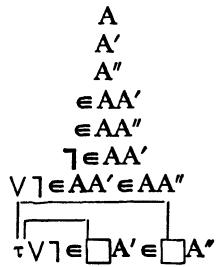
\includegraphics[keepaspectratio]{images/part001_f4a426ee2f8fe397dc0bc6599464a758ff3a832b6925cc474c9242d7de093d2f.jpg}}

Hence the assembly given as an example in no. 1 is a term in the theory of sets.*

Remark. Intuitively, terms are assemblies which represent objects, and relations are assemblies which represent assertions which can be made about these objects. Condition (a) means that the letters represent objects. Condition (b) means that if B is an assertion, then \(\neg B\) , called the negation of B, is an assertion (which is read: not B). Condition (c) means that if B and C are assertions, \(\vee BC\) , which is called the disjunction of B and C, is an assertion (which is read: either B or C); thus \(\Longrightarrow BC\) is an assertion (in words: ``either not B, or C'', or ``B implies C''). Condition (d) means that if B is an assertion and x a letter, then \(\tau_{X}(B)\) is an object. Let us consider the assertion B as expressing a property of the object X; then, if there exists an object which has the property in question, \(\tau_{X}(B)\) represents a distinguished object which has this property; if not, \(\tau_{X}(B)\) represents an object about which nothing can be said. Finally, condition (e) means that if \(A_{1}, A_{2}, ..., A_{n}\) are objects, and if s is a relational (resp. substantific) sign of weight n, then \(sA_{1}A_{2}\ldots A_{n}\) is an assertion about the objects \(A_{1}, ..., A_{n}\) (resp. an object depending on \(A_{1}, ..., A_{n}\) ).

Examples. The symbols \(\phi\) , \(\mathbf{N}\) , ``the real line'', ``the \(\Gamma\) function'', \(f \circ g\) represent terms. The symbols \(\pi = \sqrt{2} + \sqrt{3}\) , \(1 \in 2\) , ``every finite division ring is a field'', ``the zeros of \(\zeta(s)\) other than \(-2, -4, -6, \ldots\) lie on the line \(\mathcal{R}(s) = 1/2\)'' represent relations. The symbol ``3 and 4'' represents neither a term nor a relation.

The initial sign of a relation is \(\vee, \neg\) , or a relational sign. The initial sign of a term is either \(\tau\) or a substantific sign, provided that the term does not consist of a single letter. The latter assertion follows from the fact that a term is an assembly of the first species. If \(A\) is a relation, then \(A\) features in a formative construction, is not a letter, and does not begin with \(\tau\) , so that three cases are possible: (1) \(A\) is preceded by an assembly \(B\) such that \(A\) is \(\neg B\) ; (2) \(A\) is preceded by two assemblies \(B\) and \(C\) such that \(A\) is \(\vee BC\) ; (3) \(A\) is preceded by assemblies \(A_1, A_2, ..., A_n\) such that \(A\) is \(sA_1A_2 ... A_n\) , \(s\) being a relational sign.

